\documentclass[conference]{IEEEtran}

% my packages
\usepackage{url}
\usepackage{array}
\usepackage{textcomp}
\usepackage{listings}
\usepackage[T1]{fontenc} % To use quotes in listing
% \usepackage{fixltx2e}
\usepackage{subfigure,epsfig,amsfonts}
\usepackage{caption}
\usepackage{xspace}
\usepackage[usenames,dvipsnames,svgnames]{xcolor}
\usepackage{multicol}
\usepackage{graphicx}
\definecolor{codegreen}{rgb}{0,0.6,0}
\definecolor{codegray}{rgb}{0.5,0.5,0.5}
\definecolor{codepurple}{rgb}{0.58,0,0.82}
\definecolor{backcolour}{rgb}{0.95,0.95,0.92}
\usepackage{siunitx}
\usepackage{array}
\usepackage{multirow}
\newcolumntype{P}[1]{>{\centering\arraybackslash}p{#1}}

\usepackage[font={small,bf}]{caption}
\usepackage{balance} 
\usepackage{flexisym}
\usepackage{varwidth}
\usepackage{makecell}
\usepackage{float}
%\usepackage{lipsum}
\lstdefinestyle{mystyle}{
    backgroundcolor=\color{backcolour}, 
    commentstyle=\color{codegreen},
    keywordstyle=\color{magenta},
    numberstyle=\tiny\color{codegray},
    stringstyle=\color{codepurple},
    basicstyle=\footnotesize\ttfamily,
    breakatwhitespace=false,         
    breaklines=true,                 
    captionpos=b,                    
    keepspaces=true,                 
    numbers=left,                    
    numbersep=5pt,                  
    showspaces=false,                
    showstringspaces=false,
    showtabs=false,                  
    tabsize=2
}
\lstset{style=mystyle}



\newcommand{\easychair}{\textsf{easychair}}
\newcommand{\miktex}{MiK{\TeX}}
\newcommand{\texniccenter}{{\TeX}nicCenter}
\newcommand{\makefile}{\texttt{Makefile}}
\newcommand{\latexeditor}{LEd}

\newcommand{\CHIDB}{$\chi$DB\xspace}
\newcommand{\CHI}{$\chi$\xspace}
\newcommand{\TG}{\emph{T}$\!_\emph{g}$}

\usepackage[noadjust]{cite}
\renewcommand{\citepunct}{,\penalty\citepunctpenalty\,}
\renewcommand{\citedash}{--}% optionally

\newcolumntype{C}[1]{>{\centering\arraybackslash}m{#1}}
\newcolumntype{L}[1]{>{\raggedleft\arraybackslash}m{#1}}
\newcolumntype{R}[1]{>{\raggedright\arraybackslash}m{#1}}

\newcommand{\veryshortarrow}[1][3pt]{$\mathrel{%
   \hbox{\rule[\dimexpr\fontdimen22\textfont2-.2pt\relax]{#1}{.4pt}}%
   \mkern-4mu\hbox{\usefont{U}{lasy}{m}{n}\symbol{41}}}$}

\newif\ifdraft
%\draftfalse
\drafttrue

\ifdraft
  \newcommand{\ian}[1]{\textcolor{Red}{[Ian: #1]}\xspace}
  \newcommand{\roselyne}[1]{\textcolor{Blue}{[Roselyne: #1]}\xspace}
  \newcommand{\kyle}[1]{\textcolor{Purple}{[Kyle: #1]}\xspace}
  \newcommand{\logan}[1]{\textcolor{Green}{[Logan: #1]}\xspace}
  \newcommand{\debbie}[1]{\textcolor{Brown}{[Debbie: #1]}\xspace}
  \newcommand{\shrayesh}[1]{\textcolor{BurntOrange}{[Shrayesh: #1]}\xspace}
  \newcommand{\aswathy}[1]{\textcolor{WildStrawberry}{[Aswathy: #1]}\xspace}
  \newcommand{\hong}[1]{\textcolor{RoyalPurple}{[Hong: #1]}\xspace}
  \newcommand{\loganfussingaboutrecallandprecision}{\logan{<Usual noise about trading off of P for R being an artifact of meaningless thresholds. Suggestion that we need a more meaningful metric>}}
\else
  \newcommand{\ian}[1]{}
  \newcommand{\roselyne}[1]{}
  \newcommand{\kyle}[1]{}
  \newcommand{\logan}[1]{}
  \newcommand{\shrayesh}[1]{}
  \newcommand{\debbie}[1]{}
  \newcommand{\aswathy}[1]{}
  \newcommand{\hong}[1]{}
  \newcommand{\loganfussingaboutrecallandprecision}{}
\fi

\usepackage{siunitx}
\sisetup{detect-all}

% correct bad hyphenation here
\hyphenation{op-tical net-works semi-conduc-tor}

\begin{document}
% This line plus the intro lines in the Bib file concatenates author lists.
\bstctlcite{IEEEexample:BSTcontrol}

%\title{PolyNER: A \textit{word2vec} Approach to Scientific NER}
\title{Active Learning Yields Better Training Data for Scientific Named Entity Recognition}


\author{\IEEEauthorblockN{Roselyne B. Tchoua\IEEEauthorrefmark{1},
Zhi Hong\IEEEauthorrefmark{1}, 
Logan T. Ward\IEEEauthorrefmark{1}\IEEEauthorrefmark{3}, \\
Kyle Chard\IEEEauthorrefmark{2}\IEEEauthorrefmark{3},
Debra J. Audus\IEEEauthorrefmark{4}, 
Shrayesh N. Patel\IEEEauthorrefmark{5}, 
Juan J. de Pablo\IEEEauthorrefmark{5} and
Ian T. Foster\IEEEauthorrefmark{1}\IEEEauthorrefmark{2}\IEEEauthorrefmark{3}}
\IEEEauthorblockA{\IEEEauthorrefmark{1}Department of Computer Science, University of Chicago, Chicago, IL, USA\\
\IEEEauthorblockA{\IEEEauthorrefmark{2}Globus, University of Chicago, Chicago, IL, USA\\}
\IEEEauthorblockA{\IEEEauthorrefmark{3}Data Science and Learning Division, Argonne National Laboratory, Argonne, IL, USA\\}
\IEEEauthorblockA{\IEEEauthorrefmark{4}Materials Science and Engineering Division, National Institute of Standards and Technology, Gaithersburg, MD, USA\\}
\IEEEauthorblockA{\IEEEauthorrefmark{5}Institute for Molecular Engineering, University of Chicago, Chicago, IL, USA}
Email: roselyne@uchicago.edu}
}

% make the title area
\maketitle

\begin{abstract}

Despite significant progress in natural language processing, 
machine learning models require substantial expert-annotated training data to perform well in tasks such as named entity recognition (NER) and entity relations extraction.
Furthermore, NER is often more complicated when working with scientific text. 
%\logan{Perhaps move the characteristics you mention for polymers to this sentence, make them sound more general, and then say polymers is a perfect case for exploring these challenges. This will make your paper seem less polymer-y from the start}\roselyne{Making a note to ask which sentence, but have tried to add that the challenges are not usnique to polymer science}
For example, in polymer science, 
chemical structure may be encoded using nonstandard
naming conventions,
the same concept can be expressed using many different terms (synonymy),
and authors may refer to polymers with ad-hoc labels. % (in lieu of longer names).
These challenges, which are not unique to polymer science, make it difficult to generate training data, as specialized skills are needed to label text correctly.
We have previously designed polyNER, a semi-automated system for efficient identification of scientific entities in text.
PolyNER applies word embedding models
to generate entity-rich corpora for productive expert labeling,
and then uses the resulting labeled data to 
bootstrap a context-based classifier. %word vector classifier. %~\roselyne{cite in intro}.
PolyNER facilitates a labeling process that is otherwise tedious and expensive.
Here, we use active learning to efficiently obtain more annotations from experts and improve performance.
Our approach requires just five hours of expert time to achieve discrimination capacity comparable to that
of a state-of-the-art chemical natural language processing toolkit,
highlighting the potential for human-computer partnership in
%for constructing 
domain-specific scientific NER. % systems.

\end{abstract}

\begin{IEEEkeywords}
Named Entity Recognition, Machine Learning, Word Embedding, Active Learning, Polymers
\end{IEEEkeywords}

\IEEEpeerreviewmaketitle

%------------------------------------------------------------------------------
\section{Introduction}
\label{sect:apner_introduction}
A wealth of valuable research data is published in unstructured form in millions of scientific articles each year. %\cite latest version of that report?"
Reading and extracting pertinent information from those articles has
become an unmanageable task for scientists and makes
it hard to build on existing results. 
%In many fields of science, the scientific literature contains large quantities of important data in unstructured form that,
%if extracted, could benefit research.
A major obstacle to scientific fact extraction is the difficulty of identifying scientific entities in text.
Despite much progress in natural language processing (NLP), 
scientific named entity recognition (NER) remains a research challenge.
The main reason for this gap between NLP advances and scientific extraction needs is the lack of carefully annotated datasets for specific targets.
In standard NER, 
progress is made possible by, for example, the 
Conference on Computational Natural Language Learning (CoNLL) dataset,
which supports much work that advances the state of the art.
But NER systems trained on CoNNL data do not perform well for scientific text, due to 
the distinctive vocabularies used in different scientific disciplines and subdisciplines.

Science-specific training datasets have been established in
%Efforts have been launched 
%In contrast, there is a conference organized around the CoNLL dataset for standard NER and other NLP tasks to push the state-of-the-art each year.
%Driven by bioinformatics\textemdash which develops methods and software tools for understanding biological data\textemdash similar efforts exist in 
biology~\cite{song2004posbiotm} and, more recently, chemistry~\cite{krallinger2015chemdner}.
However, the expert effort required to 
design 
%complete 
extraction schema, 
define clear annotation rules, and generate training data % for most advanced machine-learning based NLP techniques 
is substantial, and cannot feasibly be performed for 
%has to be repeated for 
every field of science.
%\logan{Are you sure you want to use materials science as the opening line? Maybe add a general sentence up top "data-intensive science is awesome, but requires accessible data. The development of new materials is a great example for such opportunities and needs in domain science. [I'm making these comments under the context that this will be a thesis chapter]}\roselyne{point taken!}
As a consequence, annotated datasets do no exist in most fields,
%In many fields, such as material science, no such annotated datasets exist.
preventing the application of state-of-the-art NER and fact extraction methods.

%This problem is apparent in materials science where, 
%despite many publications containing much data,
%a lack of annotated datasets impedes progress in materials informatics, 
%a field that aims to replace current trial-and-error materials design processes
%by combining large datasets and computational models to achieve targeted materials design, 
%thus reducing time-to-market and development costs of new materials.

This problem is apparent in materials science, where materials informatics 
seeks to combine large datasets and computational models to 
replace current trial-and-error materials design processes with targeted materials design, 
thus reducing time-to-market and development costs of new materials.
A lack of annotated training data has hindered progress,
preventing large-scale application of methods pioneered in, for example,
biomedicine.
Those methods, which often use hybrid rule-based, machine learning, and statistical techniques to extract entity names and relations from the literature~\cite{leaman2008banner,zeng2015survey}, require much training data.
%the process of designing new materials is still one of trial and error.
%The field of materials informatics aims to address this problem by combining large datasets and computational models to achieve targeted materials design and reduce time-to-market and development costs of new materials.
%A large amount of such data already exists in unstructured text in the scientific literature, but the lack of training data impedes the direct application of state-of-the-art extraction methods.
% hence the need for materials information extraction.
%\logan{Good intro paragraph. "Opportunity -> problem you are solving" in an inch of text}\roselyne{Thanks!|}
%There is a considerable amount of prior work in scientific facts extraction, notably in biomedicine. 
%State-of-the-art methods often use hybrid rule-based, machine learning, and statistical techniques to extract entity names and relations from the literature~\cite{leaman2008banner,zeng2015survey}. 
While similar efforts have begun in materials science~\cite{hawizy2011chemicaltagger,rocktaschel2012chemspot,leaman2015tmchem,swain2016chemdataextractor,young2018data}, the lack of available training data for new materials impedes rapid progress. 
Instead, each new research project targeting a new type of materials must first undertake considerable
effort to create a large, carefully annotated training
data tailored for this new target, a task that often requires considerable in-depth domain knowledge.

The subfield of polymer science puts these problems in particularly stark relief.
Polymers have their own unique nomenclature, as we explain below, and thus annotated datasets created for general
chemistry are of little value.
Scientists and engineers lack access to a freely available large database of polymers and their properties.
%\kyle{should cite our previous papers about polyNER. ANd change phrasing here to make it sound like polyner is now well established
%and what we are doing here is enhancing it with active learning. }
To address these challenges, we have previously designed polyNER, a system for generating training data for scientific NER using semi-supervised and active learning.
PolyNER uses NLP to produce sets of candidate entities, which
experts 
%iteratively 
approve or reject via a 
%easy-to-use 
Web interface;
%in small batches selected using an active learning
%\ian{You say that polyNER uses active learning, then you say that you enhance it with AL in this paper. 
%Inconsistent?}\roselyne{yes thank you, made some changes (too fast) after Kyle pointed out that we had already introduced polymer in the now accepted paper}.
% approach;
the resulting labels are used to train context-based word vector classifiers. %after each round.
PolyNER's labels can also be used to train other machine learning models to leverage other features in addition to context, such as word morphology
to recognize target entities.
%\ian{The reference to ``beyond their context'' doesn't make sense to me; I wonder if it will to other readers.}
The goal is
to substitute the labor-intensive processes of assembling a large
manually annotated corpus (and reduce costs) by using small numbers of carefully selected candidates to be labeled via focused expert input. 

In this paper, we seek to improve polyNER's performance by improving the labeling process and the classification of entity word vectors. 
%\ian{I note that in the architecture section, you refer to this phase as sampling, so I changed 
%the text in the results section to be consistent. Not sure if you want to change here too, or change other secitons back,
%but should be consistent.}
%labeling, and classification.\ian{Classification is not shown as a step elsewhere. Also, I note that Figure~1 has a
%``candidate discrimination'' step, which is a term not used much elsewhere.}\roselyne{Noted! I changed figure 1 and will check that we don't use discrimination elsewhere. Also remove any mention of the candidate generation since now we only do it at the initial labeling.}
In the initial labeling phase, 
we experiment with different \textit{representative} (commonly used) entities to increase the fraction of target entities in the dataset to be labeled and bootstrap the context-based word vectors classifiers. %\ian{I think that the representative/seed entity thing is mainly relevant for bootstrapping. Maybe we should say ``used in the bootstrapping phase.'''}
 % to generate candidates;
% and tune the word embedding model parameters to increase the yield of actual scientific entities among candidates; 
In the subsequent labeling and classification steps,
%\ian{is this rewording correct? I think that as you say you improve each step,
%you should be explicit about what you did to improve in each step.}\roselyne{yes correct}
we use active learning with maximum entropy uncertainty sampling and two different pools of unlabeled data to train classifiers, and compare their learning rate after five rounds. 
%\logan{"seed entities" is not a standard term, right? If it is not standard, maybe use something less metaphorical "ways to generate initial candidates for labeling"}\roselyne{I don't think so standard but I picked it up from similar works in NER, snowball, do you mean not to use it in the intro or the whole paper. Will search and see how many times I use it. I had started using representative entities, which I also have to define.} 
Using labels generated via active learning, we train word vector classifiers and achieve NER performance comparable to 
a modified version of a state-of-the art rule-based chemical entity extraction
system, ChemDataExtractor (CDE)~\cite{swain2016chemdataextractor}.
We have previously enhanced CDE
with dictionary- and rule-based methods for identifying polymers~\cite{tchoua2017towards}.
%\ian{It is not clear, I think, whether you are comparing against the regular CDE or the enhanced CDE. Should you compare against both?}\roselyne{CDE is extracting all chemicals, we actually achieve higher recall which could be an important result, but doesn't it complicate explanations?}
Our system, however, took five hours of expert time to achieve this result.
%\ian{We mention five hours repeatedly, sometimes saying five hours, sometimes less than five hours, sometimes $sim$ five hours. I think we should mention it less often, and be consistent in how we phrase it.}

The rest of this paper is as follows. 
In Section~\ref{sect:background}, we motivate the need for identifying polymer names in
text. 
We review semi-supervised methods for NLP systems in
Section~\ref{sect:apner_related}. 
We describe the design and implementation in Section~\ref{sect:apner_architecture} and evaluate polyNER
in Section~\ref{sect:apner_results}. We summarize and discuss future work in Section~\ref{sect:apner_conclusion}.
%\logan{<soapbox>I only see CS have this "table of contents" paragraph. Is it explicitly required, or just an idiosyncrasy of the CS community? Also, does everyone skip over them while reading anyway?</soapbox>}\roselyne{Very common in computer science paper I think, I'll let Ian and Kyle confirm.}
%------------------------------------------------------------------------------

%------------------------------------------------------------------------------
\section{Motivation}
\label{sect:background}
%\roselyne{Adjust/shorten since I added text.}
%\kyle{Sounds similar to previous paper. First paragraph should be re-written.}
%\roselyne{Yes, it's exactly the same! Made a note to myself but hadn't come back to it yet.}
%\ian{This is the first reference to ``chemical NER,'' which you have not previously said you are addressing: 
%above, you refer to materials science.}\roselyne{mistake, I think I can directly say polymer science here, or have a different intro}
Our work is generally motivated by the need to extract previously unmined scientific entities;
our initial goal is to enable machine-learned extraction of polymer names. 
The challenges of polymer science NER are similar to those in biomedicine~\cite{krallinger2015chemdner,kim2004introduction}. 
Entities can be described with multiple referents (synonymy).
Conversely, the same word may refer to different concepts depending on context (polysemy).
For example,
\textit{polystyrene} is often referred to as \textit{PS}, but \textit{polystyrenes} can also be referred to as \textit{GPPS}, \textit{HIPS}, and \textit{EPS}; combined with other monomers yielding \textit{SBR}, \textit{SBS}, and \textit{ABS}; or used to describe polystyrene derivatives such as \textit{PAMS}, \textit{PMS}, and \textit{PSS}.
%\textit{Polystyrene} is often referred to as \textit{PS}, but \textit{polystyrenes} also describes a family of polymers including \textit{GPPS}, \textit{HIPS}, \textit{EPS}, \textit{SBR}, \textit{SBS}, and \textit{ABS}. 
%\roselyne{Ask Debbie to check previous example. Done!}
While standards for naming polymers exist (e.g., International Union of Pure and Applied Chemistry (IUPAC~\cite{hiorns2013brief}) naming conventions), they are not always followed in practice~\cite{tamames2006success}. 
Instead, polymer names may be reported as source-based names (based on the monomer name), structure-based names (based on the repeat unit), common names (requiring domain specific knowledge), trade names (based on the manufacturer), and names based on chemical groups within the polymer (requiring context to fully specify the chemistry), generating variability in naming conventions.
Typographical variants (e.g., alternative uses of hyphens, brackets, spacing) and alternative component orders cause more variations between polymer names in the literature.
The origin of these different naming conventions is linked to the desire for clarity within a journal article, coupled with the often-complicated monomeric structures~\cite{audus2017polymer}.
%For example, sequence-defined polymers, where multiple monomers are chemically bound in a well-defined sequence as in proteins, often defy normal naming practices as it is not possible to concisely list every monomer and the respective position of the monomer~\cite{lutz2014polymer}. 
%Another class of polymers that often suffer from complicated names are conjugated polymers, which exhibit useful optical and electrical properties. 
%Conjugated polymers are complex due to the co-polymerization of multiple monomers (donor/acceptor units), the type and position of side chains along the polymer backbone and the coupling between monomer units to control regioregularity~\cite{himmelberger2015engineering}.

In addition to challenges related to the makeup of the scientific entities, the scarcity of entities in scientific literature and the lack of training data also impedes the use of recent machine learning based NER techniques.
%\logan{I don't know the word "paucity." Am I just unread, or should we use a lower-brow word?}
%\roselyne{I need to admit you made me google the term lower-brown word :-) will use scarcity, or sparseness or rarity?}
Considerable time and manual effort are involved in creating and maintaining the balanced
CoNLL dataset for standard NER~\cite{tjong2003introduction}.
Example sentences from such corpora include one or more entities per sentence. 
In our attempt to recognize polymer names in full text documents, we face a very imbalanced dataset where most sentences do not contain a target entity, as there are only a handful of target entities per document.
%(we found less 2\% of words in sample publications are polymers in our test dataset)
While there has been much interest in machine learned recognition of biochemical entities~\cite{jessop2011oscar4,rocktaschel2012chemspot,leaman2015tmchem,swain2016chemdataextractor}, 
the successes that have been achieved have required much human effort to generate quality training data~\cite{krallinger2015chemdner}.
%\ian{``there has concurrently been significant effort involved in selecting...'': 
%can we say simply, ``the successes that have been achieved have required much human effort to
%generate quality training data~\cite{krallinger2015chemdner}.''? 
%The current text seems to me to be oblique and also to imply that it may be possible to generate training
%data \emph{without} manual effort.}
%there has concurrently been significant effort involved in selecting and (often manually) generating quality data for
%trainable statistical NER systems~\cite{krallinger2015chemdner}. 
Previous work has also found that even state-of-the-art NER systems do
not typically perform well when applied to different domains~\cite{krallinger2013overview}. 
Therefore, the problem of training machine learning models to recognize new scientific entities in a new field, such as polymer science, remains challenging.




%------------------------------------------------------------------------------

%------------------------------------------------------------------------------
\section{Related Work}
\label{sect:apner_related}
NER and other information extraction tasks rely on large amount of training data, which are expensive to obtain.
Weakly supervised learning methods work with much less training data and aim to address this challenge.
They generally fall under two categories: semi-supervised learning and active learning~\cite{zhou2017brief}.
The key difference between the two is that the former relies on approximately labeled data (as opposed to correctly labeled data for supervised learning) and the latter starts off with unlabeled data.
Semi-supervised learning attempts to label data automatically by using prior knowledge and a set of labeled data. 
For example, it assumes that if $x$ and $y$ are similar, they probably have the same label (first cluster the whole dataset, then label each cluster with labeled data~\cite{zhu2005semi}).
%\ian{The reference to ``cluster and label algorithms'' is obscure to me.}\roselyne{Does the sentence still make sense to you without that ``hint'', the idea is to cluster the data and assign }
%\kyle{Could be a clearer description of semi-supervised learning}\logan{Agreed. The key thing that separates it from other learning is that it uses labeled and unlabeled data}\roselyne{Added key difference explicitely as suggested}
Active learning assumes there is a source of knowledge, such as a human expert, that can be queried 
to label a selected batch of unlabeled data. 
%\logan{It sounds like these two categories are mutually exclusive. Do you think so? Can you state what differentiates them explicitly?}\roselyne{I think maybe one key element in polyNER is that we combine the two, we start of with approximate labels (distance labels), then continue with active learning) but I don't think I am the only one doing this, have found other examples scheming papers, like clustering and doing active learning across previously clustered data}

\subsection{Semi-supervised Approaches}
\textit{Bootstrapping} is a semi-supervised technique, which starts from a small set of seed relation instances and iteratively learns more relation instances and extraction patterns.
Snowball~\cite{agichtein2000snowball} which improved the DIPRE system~\cite{brin1998extracting}, used an intuitive idea to collect new entity relations using a set of seed entity pairs.
In the DIPRE system, the intuitive assumption is that, given a few seed entity relations, the text between two known target entities in close proximity of each other describes and consistutes a \textit{pattern} of the relation between the two. 
Since that is not the case in practice, the system uses a limited set of regular expression to limit useful patterns, hence decreasing the number of false positives.
A key improvement of Snowball
is that its patterns include named-entity tags (PERSON, LOCATION, ORGANIZATION, etc.).
Given a handful of seed tuples of ORGANIZATION and LOCATION, Snowball attempts to learn the relation \textit{HeadquarteredIn} by assuming that each time the tuples appear in close proximity to each other, 
the text in between illustrates the desired relation.
This text can then be used to discover new tuples, which can in turn be used as seeds for the next discovery iteration.
Of course, organizations may be located but not headquartered in multiple cities;
hence it is important to inspect the quality of extraction patters to reduce noise in the generated output.

\textit{Distant supervision} maps known entities and relations from a structured knowledge 
base onto unstructured text~\cite{peters2014machine,de2016deepdive}. 
With freely available structured knowledge base such as DBPedia~\cite{auer2007dbpedia} and Freebase~\cite{bollacker2008freebase}, it is possible to leverage a large set of known entity pairs to generate training data.
%~cite{mintz2009distant}; 
%in this work authors assume that if two entities participate in a relation, any sentence that contains both entities descripes that relation. 
%Because that is not always the case, they extract features from different sentences to define
%lexical, syntactic and named entity tag features. 
%They use standard multi-class logistic regression as the classification algorithm and reach almost 70\% of precision based on human judgment.
Over the past decade, probabilistic approaches have been proposed to allow automatic selection.
For example PaleoDeepDive~\cite{peters2014machine}, built upon DeepDive~\cite{de2016deepdive}, automatically extracts
paleontological data from text, tables, and figures in scientific publications. 
For good performance, such approaches often rely on and extend large databases: for example,
PaleoDeepDive uses PaleoDB~\cite{PaleoDB}. 
The system labels any entity pair that appears in the database as \textit{True}.
The user defines features (e.g. if a specific keyword appears between two entities, that pair a certain attribute is labeled \textit{True}, but if the entity pairs are too far apart, another attribute is marked \textit{False}, 
%\kyle{I don't get how this is an example feature. Seems like its more labels.}), \roselyne{Hope it's clarified, they're more like user defined functions and rules - this is Snorkel's ancestor}
the system then uses statistical inference to determine the probability that each newly discovered pair of interest is \textit{True}.

\textit{Data programming}, as used in the Snorkel system, has users define 
\textit{labeling functions} to provide labels for data subsets~\cite{ratner2016data}. 
Errors due to differences in accuracy and conflicts between labeling functions are 
addressed by learning and modeling the accuracies of the labeling functions. 
Under certain conditions, data programming achieves results on par with those of supervised learning methods.
While writing concise scripts to define rules may seem to be a more reasonable task for annotators 
than exhaustively annotating text, it still requires expert guidance.  
In data programming as in boostrapping and distant supervision it is important to evaluate the quality of functions and extraction patters to decrease noisy patterns.

\subsection{Active Learning}
Active learning~\cite{zhou2017brief} assumes that gold standard labels for unlabeled instances can be obtained by
querying an oracle (domain expert or source of knowledge).
The goal of active learning is to decrease labeling costs by requesting a limited number of labels from the oracle, that have been deemed most valuable by the learner.
Uncertainty sampling approaches define ``valuable'' data by measuring uncertainty in the predictions.
For example, in the case of a single learner, querying predictions with maximum entropy in which the learner assigns all classes with equal probability~\cite{lewis1994heterogeneous} or predictions closest to the decision boundary in the case of support vector machine classifiers~\cite{campbell2000query}.
In the case of multiple learners, query-by-committee requests labels for unlabeled instances on which the learners disagree the most~\cite{seung1992query}.
Uncertainty sampling and query-by-committee are representative approaches based on informativeness, where informativeness measure show well an unlabeled instance helps reduce the uncertainty. 
Another selection criterion addresses representativeness, which measures how well an instance helps represent the structure of input patterns; in this case selection is made by querying data from unlabeled clusters of data~\cite{nguyen2004active,dasgupta2008hierarchical}.


\subsection{Placing polyNER in Context}
%\ian{I feel that it is clearer to have a subsection here. Also: I think the goal is to put polyNER in context, but I am not sure that it does so clearly, yet. It seems to me to be currently a rather hard-to-follow statement of the polyNER approach, which I would expect to find elsewhere.}
%\roselyne{This was a subsection, but was removed as some found it strange here, but the purpose was indeed to relate polyNER to the previous paragraphs, giving it a second read.}
%\roselyne{The main purpose also was to indicate that there was already work on polyNER and we are extending the work here}
PolyNER extends previous work to create a low-cost scientific fact extraction system. 
%We ask: how can we quickly generate annotated data for scientific named entity recognition?
Specifically, we address two challenges: 
(1) lack of (expensive) training data in some fields, including our own polymer science application which lacks free access to large polymer databases; and 
(2) the need for domain expert curators, which impedes the use of crowdsourcing platforms such as Amazon Mechanical Turk~\cite{buhrmester2011amazon} or Figure8~(\url{https://www.figure-eight.com/}).
\ian{I find it odd that we are introducing the challenges that polyNER addresses here. It seems that we have
already done that, to some extent, in the introduction and the background. Ideally that would be in one place.}
\roselyne{Come back to this, after rereading intro and intro to architecture. This was supposed to clearly separate polyNER form the other systems.}
%\ian{The text alternates between third person and first person. Maybe be consistent third person: ``The polyNER approach ..." not ``our approach"?}
PolyNER has in common with prior work that it combines semi-supervised and active learning~\cite{nguyen2004active,basu2004active}.
%\ian{In the intro, the three stage are named candidate generation, labeling, and classification. Perhaps use those terms here too?}
In the first phase, the candidate generation is similar to bootstrapping but applied to named entities rather than entity pairs. 
%\logan{Confusing. If PolyNER is similar to bootstrapping, why are are you describing it in the active learning section? I'm generally not sure why this paragraph is in "Related Work"}\roselyne{This was its own section, related polyner to all previous sections including bootstrapping and not just active learning, but felt a bit weird to Kyle, so we moved it to motivation, perhaps it fits before current changes to architecture to motivate what we are doing now. Will just try to do this link between our work and related work in each section and have a polyNER paragraph in architecture.}
%\ian{I want to confirm that the next sentence is correct. It states that you generate approximate labels by extracting
%words similar to seed entities, implying (to me) that this process somehow generates labels (automatically?). I thought this was the
%candidate generation phase.}
The initial batch of labels contains strings deemed \textit{similar} to a few seed entities, 
with similarity determined by using word representations and vector distance measures.
%\ian{In the next sentence, I have no idea what ``noise in the output'' means, and I wonder if other readers will?}
As this approach is approximate and is likely to include errors (words that have similar context to entities but are not actual entities), the next phase is expert labeling. 
Subsequent batches of labels are obtained via active learning and used 
%To address noise in the output, expert label small batches of candidates, 
%which can be used\ian{the term ``can be used'' confuses me. Is the training that is defined here part of your system?}
 to train a context-aware word vector classifier in the last phrase.
%\ian{what does ``final'' mean?}\roselyne{the idea here is that candidates from the candidate generation phase are loosely labeled polymers, but subsequently corrected by experts, the real assignments are done at the classification. Will rephrase.}
%scientific named entities.
%\kyle{Somewhat hesitant to include the next sentences. Doesnt feel like it belongs here}\roselyne{I think it's ok here if we're trying to emphasize how it is different, but I guess you want to phrase it as a contribution and it may need to be repeated in the intro/conclusion. Making a note for tomorrow}
PolyNER can be used in a way that complements other scientific NER approaches. 
For example, it could be used as a scientific entity tagger (i.e., recognizer) to be used with data programming to extract polymer properties.
%PolyNER could provide a scientific entity tagger (i.e., recognizer) to be used with data programming to extract polymer properties.\ian{I am not sure what this sentence is here for. I think that you are trying to explain how polyNER can 
%complement other approaches. If so, then how about a paragraph that speaks to that directly. E.g., ``PolyNER can be used in a way that complements other scientific NER approaches. For example, it could be used as a scientific entity tagger (i.e., recognizer) to be used with data programming to extract polymer properties.}
%An example rule could be defined as: \textit{if a sentence contains a polymer name and the words ``glass transition,'' then extract number(s) in the sentence as potential glass transition temperature(s) for that polymer.}
%We discuss the architecture of our system in more details in the next section.
%------------------------------------------------------------------------------

%------------------------------------------------------------------------------
\label{sect:apner_architecture}
\section{Design and Implementation}

PolyNER uses word representations and minimal domain knowledge (a few
seed entities) to produce a small set of candidates for expert labeling;
labeled candidates are then used to train named entity word vector classifiers.
We implement an active learning loop in order to incrementally improve the performance of the classifiers.
In order to explore whether natural language processing, and specifically the use of word vector coordinates as features can accelerate the learning process,
we use three sampling strategies and two different candidate pools for maximum entropy uncertainty sampling, which we describe in this section.
The general architecture of polyNER is illustrated in Figure~\ref{fig:architecture}.
We also describe the labeling process, and training and testing configuration for our word vector classifiers in the active learning loop. 

\begin{figure*}[!t]
{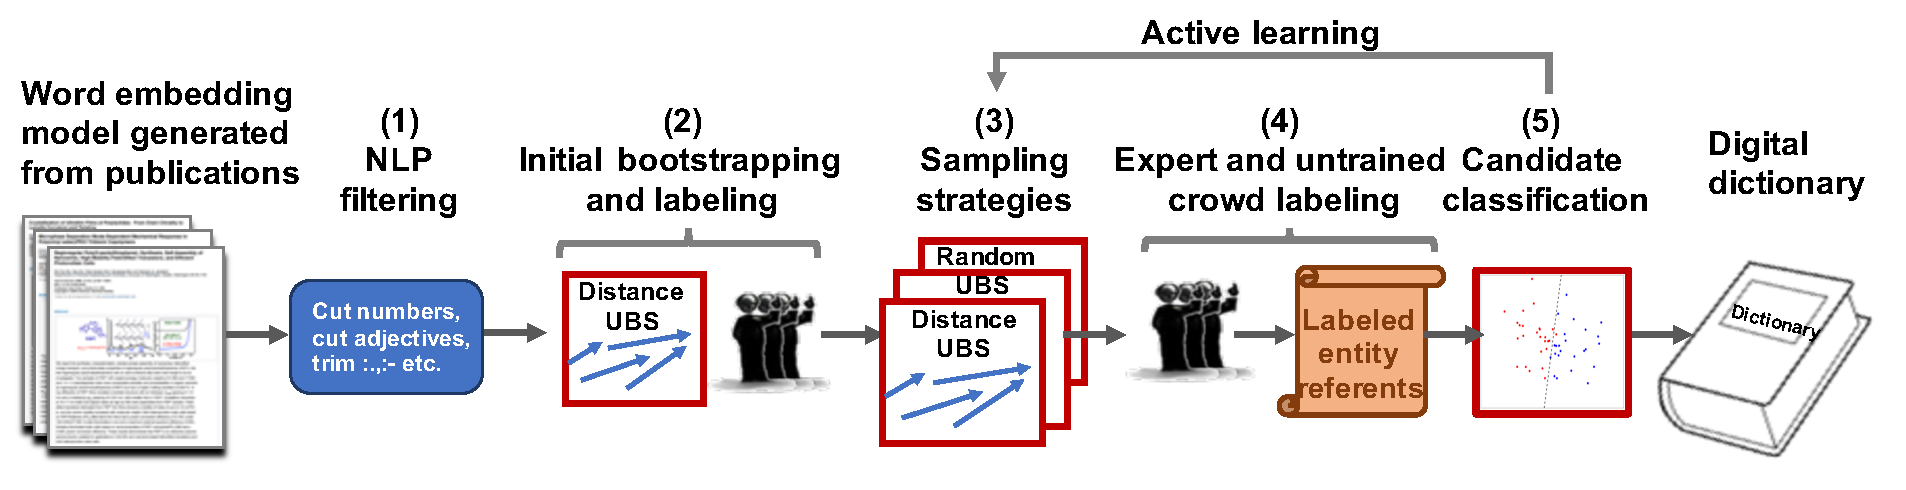
\includegraphics[width=\textwidth]{figures/architecture.pdf}}
\caption{\label{fig:architecture} PolyNER system showing NLP-filtering in (1), candidate sampling strategies in (2), and actie learning loop between expert labeling (3) and classification of scientific named entities (4). 
%\kyle{Would be good to have some more padding on the NL filtering step. Also not sure ``cut numbers, vocab'' is meaningful? Sampling strategies has the m from random on the second box. Again, maybe some padding there would be clearer.}\roselyne{shrank some text and fixed the vocab term.}
}
\end{figure*}

\subsection{Preprocessing}
First, we define an
NLP filtering preprocessing step that is used to filter out
words in scientific publications that are unlikely to be polymer referents. 1) We remove numbers. 2)
Hypothesizing that names of scientific entities will not, in general, be English
vocabulary words, we remove words found in the SpaCy dictionaries
of commonly used English words~\cite{choi2015depends}. (We manually remove common polymer
names, such as polystyrene and polyethylene, from the dictionaries.) 3) We use
SpaCy's part-of-speech tagging functionality to remove non-nouns. 4) We remove
unwanted characters (e.g. `:', `.', `,', `:', `-') from the beginning and the end of each
candidate, allowing us to recognize, for example, polyethylene; (which fails the
exact string comparison test against ``polyethylene''). 5) We remove plurals (e.g.,
polyamides, polynorbornenes), as they can represent polymer family names.
We refer to these pre-processed words (output of step 1 in Figure~\ref{fig:architecture}) as NLP-filtered candidates.



\subsection{Labeling Strategies}
%\kyle{We should think about how to structure this. It seems like we want to outline
%the normal process and then perhaps introduce some baselines for comparison in the next section.}\roselyne{I'll leave this here and make a note to talk but I think we don't have much to gain comparing these since we started them all with the distance candidates. Hope it still makes sense this way.}
While the previous steps reduces the numbers of candidates and the imbalance of the dataset (target vs. non-target entity ration), there still remains a relatively large pool of potential candidates to select entities from.
In order to achieve higher classification accuracy\textemdash
by decreasing the number of potential false positives (candidates incorrectly identified as targets by our classifier)
\textemdash we want to carefully select examples to be labeled by experts.
%\kyle{I feel like some linkage is needed here. You should define what the purpose of these labeling strategies are. 
%The idea being that from the large pool of potential candidates we have to pick a set of candidates for labeling
%that we hope will give us a broad training set for improving accuracy of the classifier. }
%\kyle{Should define how we do the first selections when we have no information.}\roselyne{I think this is hard to do without first describing the AL2 strategy. I think I mention it in the results section.}
%\kyle{Also is the figure wrong. Aren't the sampling strategies part of the active learning loop?}\roselyne{yes they are part of the loop, I've added that so that there is a link between this and the next figure}
We implement three sampling strategies, which we refer to as \textit{Random}, \textit{Active Learning 1 (AL1)} and \textit{Active Learning 2 (AL2)}, 
to determine which candidates to label.
Based on preliminary experiments, we set the size of batches of strings to be labeled to 200 or about an hour of expert time.

\subsubsection{Random Strategy}
In the first strategy we randomly select 200 out of the pool of unlabeled NLP-filtered candidates.
Note that the imbalance between polymers and other \textit{tokens} (words or space separated strings) that 
do not exist in in this set is still significant (less than 5\% in our test set).

\subsubsection{Active Learning using NLP-Filtered Candidates (AL1)}
In the second strategy we use maximum entropy sampling method using the same pool of unlabeled NLP-filtered candidates.
As previously mentioned, maximum entropy selection falls under the category of uncertainty sampling, which identifies data points where a classifier predicts outcome at the decision boundary between two or more classes. 
For example, in our case, when predicting whether a word vector represents a polymer, or not, the classifier assigns equal probability to either case.
In the binary case, probabilities range from $0$ to $0.5$. Therefore, we predict outcome for all our NLP-filtered candidates and obtains a probability $p$ for each data point. We compute a list of $0.5-p$ values for all unlabeled data and sort the list in ascending order.
Points with scores closest to $0$ are most uncertain, we select the first 200 entries from this ordered list to be labeled by experts.

\subsubsection{Active Learning using NLP-Filtered Distance Candidates (AL2)}
\kyle{Calling them AL1 and 2, is hiding the fact that they are quite different. Could we instead do something like Prediction Certainty and Context Similarity? I'm sure we can come up with a better name even.}
Finally, the third pool is composed of NLP-filtered candidates deemed to be most similar to seed entities using vector similarity measures.
The intuition behind generating this pool of candidates is to increase the likelihood that a candidate is a target referent (name, acronym, synonym, etc.) by comparing its vector to that of a known entity.
Our goal is to determine whether polymers are used in a consistent context that can be used to detect and classify their corresponding context-aware vectors.
For example, the polymer name ``polystyrene'' in a sentence ``The
melting point of polystyrene is ...'' suggests that X may also be a polymer in the
sentence ``The melting point of X is ...''.
A word embedding method maps each word
in a sentence or document to a vector in an n-dimensional real vector space
based on the linguistic context in which the word appears. (This mapping may
be based, for example, on co-occurrence frequencies of words.) 
We can then
determine the similarity between two words by computing the distance between
their corresponding vectors in the feature space.
We use Word2Vec, a recent, light-weight and easy-to-use implementation of context-based vector representations~\cite{mikolov2013efficient,mikolov2013distributed}.
Specifically we use the Gensim continuous bag-of-words
(CBOW) implementation of the Word2Vec
algorithm~\cite{rehurek2010software} to generate vectors.
We can then determine, for each NLP-filtered word, the extent to which it occurs
in a similar context to the representative polymers, by computing the similarities
between the word's vector and those for our seed entities. 
When dealing with multiple seed entities, we use the highest similarity score for ranking candidates.

\begin{figure*}[!t]
\centering
\scalebox{0.6}{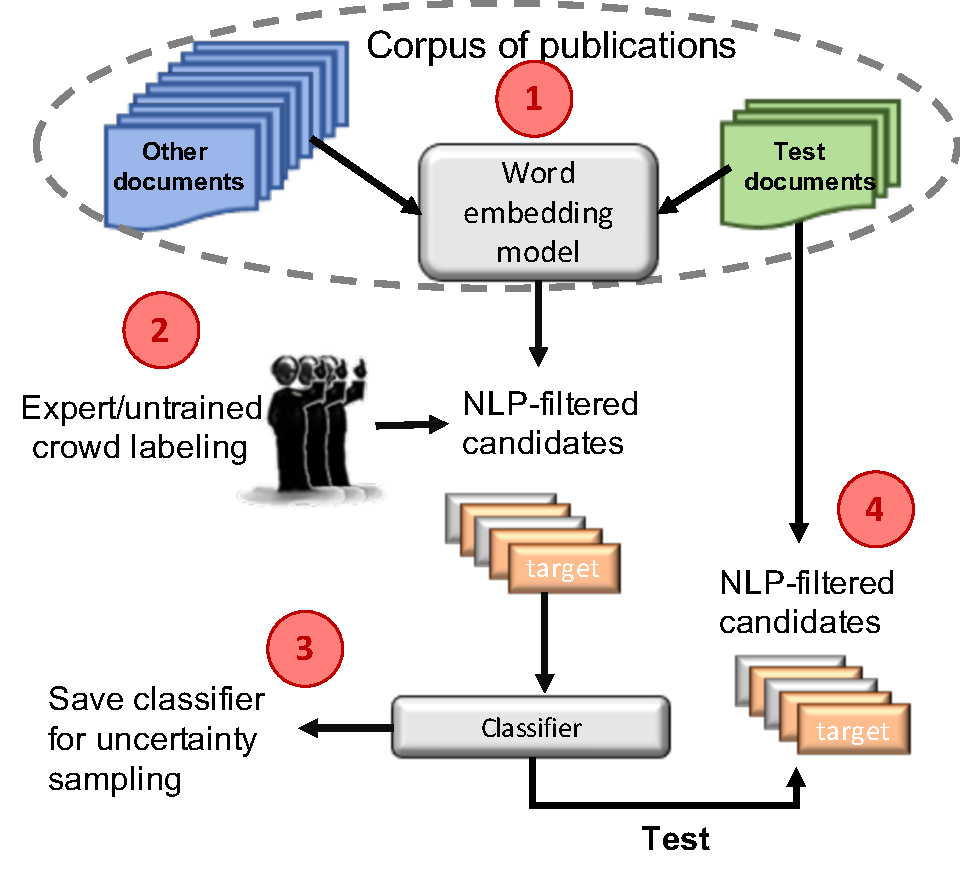
\includegraphics{figures/al_setup.pdf}}
\caption{\label{fig:current} The active learning experiment set up; we generate an unsupervised word embedding model using our entire corpus in 1), we propose NLP-filtered candidate entities to untrained and expert annotators in 2) before classifying their word vectors in 3). We save this classifier for uncertainty-based selection of labels for the next round of active learning. In 4), we test this word vector classifier on all NLP-filtered words from the test documents.}
\end{figure*}

\subsection{Active Learning Loop}
Without prior knowledge of the distribution of target entities in the vector space, we use multiple of classifiers at each iteration of the active learning process. 
We save the best performing classifier on the labeled candidates for subsequent maximum entropy-based uncertainty sampling. 
The requested labels are annotated by humans to serve as addition training data for the next learning iteration. 
We describes these steps in more details in the following sections.

\subsubsection{Word Embedding Model}
We hypothesize that we can implement a classifier, which can detect word vectors for polymers based on their context. 
We generate an unsupervised word embedding model using out entire corpus and train classifiers on vector representations using labels generated via the active learning(step 3 of Figure~\ref{fig:current}).
Finally, in step 4, we test our classifiers against all the NLP-filtered words from the test corpus, as shown on Figure~\ref{fig:current}.

\subsubsection{Untrained and Expert Labeling}
As explained in section~\ref{sect:background}, recognizing polymers can require more or less domain expertise.
We assign two domain experts to annotated candidates generated using our two maximum entropy-based uncertainty sampling (\textit{AL1} and \textit{AL2}). 
Each expert annotates one strategy but we perform crosschecking for 10\% of the first batch of labels. We confirm agreement between labels for all but 1 of the set of 20 candidates or an agreement of 95\%.
Experts simply approve or reject candidates using a simple web interface shown on Figure~\ref{fig:polyner}; a task that is more efficient than reading and annotating words in text.
The interface
provides example sentences as context for ambiguous candidates,
and allows the expert to access the publication(s) in which a particular candidate
appears when desired.

Expert time is costly and we aim to reduce the cost of obtaining labels.
Therefore for our baseline of randomly sampled NLP-filtered nouns, we experiment with a two-phase review process.
Tokenization can be a challenge for scientific entities such as polymers which contains characters such as `:', '\textendash', `,' etc. It can also generate other incoherent tokens from text, equations, captions etc.
For example, an untrained annotators may recognize that `$d\Sigma/d\Omega)(Q$' is not a polymer name and save time for the experts.
Hence, we assign two graduate student labelers to curate the candidates generated by the random sampling strategy, which is less likely to contain target entities.
First, the untrained labelers rejects obvious non-candidates via the previously mentioned web interface. 
Next, one of our expert polymer scientists indicates, for each remaining
candidate, whether or not it is in fact a polymer referent and submits a final review.
While we first used this two-phase review process for the random strategy, we envision generalizing and leveraging humans with different expertise through multi-phase reviews for all strategies to further save future costs.
%\kyle{Here we might want to think about positioning this as 2-phase review where we combine humans with different expertise levels}\roselyne{That's what I try to write about, I will specify that we did this for the random strategy but it could be applied to all strategies}


\begin{figure}
\centering
\frame{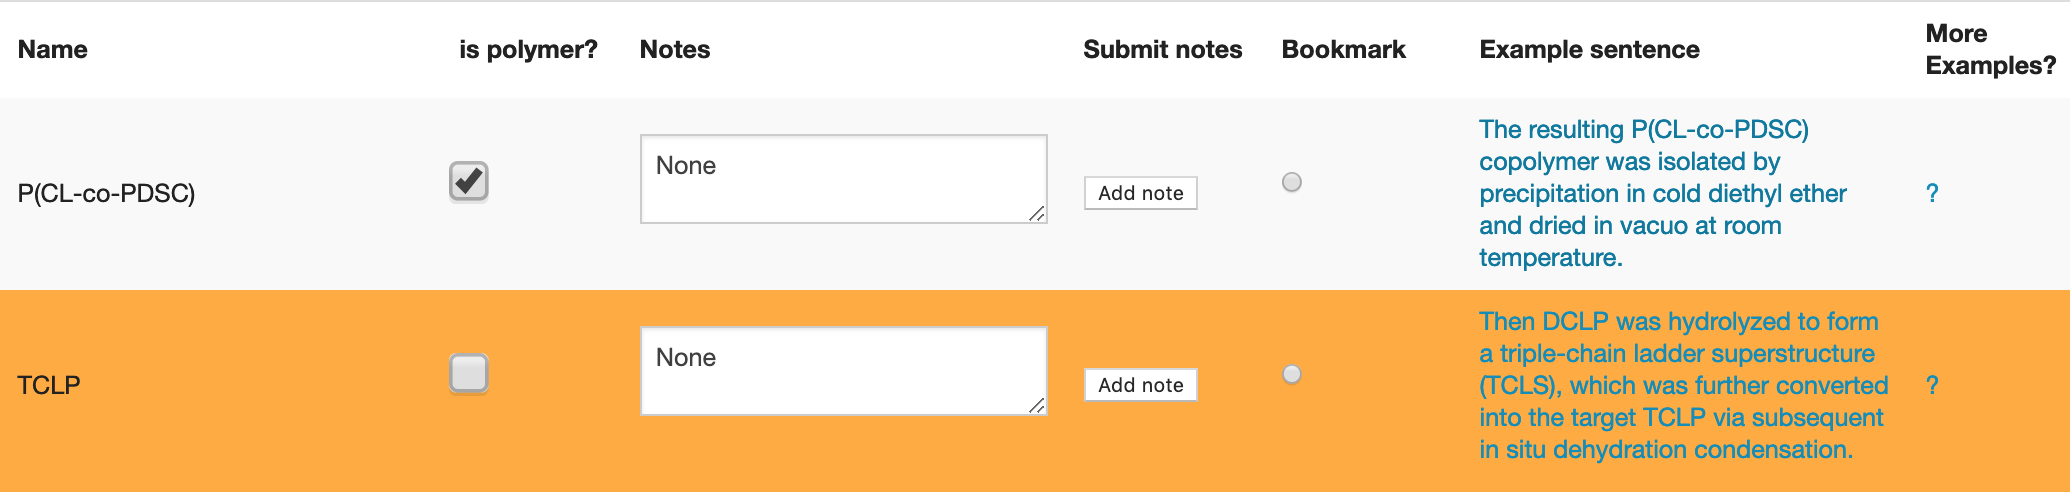
\includegraphics[trim=0in 0.1in 0.1in 0.in,clip,width=3.5in]{figures/expert_labeling.png}}
\caption{\label{fig:polyner} Web interface showing annotated candidates.
Clicking on ``?'' delivers up to 25 more example sentences.
}
\end{figure}

\subsubsection{Classification or Candidate Discrimination}
We use multiple of classifiers that we concurrently trained and test on the same data in steps 1, 2 and 3 illustrated on Figure~\ref{fig:current}.
The classifiers include the scikit-Learn implementations of Decision Tree (DT), Gradient Boosting (GB), K-Nearest Neighbor (KNN(uniform and distance weights)), Logistic Regression (LR), Linear Support Vector Machine (SVM), Naive Bayes (NB), and Random Forest (RF)~\cite{scikit-learn}. 
Our goal here is to explore the word embedding space and determine which classifier(s) works best for detecting our scientitic named entities.
As previously mentioned, we save the \textit{best-performing} classifier on labeled candidates (prior to updating the word embedding model  with test documents in order to clearly separate the training process from the test set, see step 1 in Figure~\ref{fig:current}).
When defining best performance, we prioritize retrieving a maximum of targets over precise extraction.
In other words, extracting a higher number of targets potentially requiring additional curation is favored over fewer correct targets.
In each case, we use the dimensions of the word vector for each string as input features.





%------------------------------------------------------------------------------

%------------------------------------------------------------------------------
%\section{Parameter Study}
\label{sect:parameter_study}

%------------------------------------------------------------------------------

%------------------------------------------------------------------------------
\section{Evaluation}
\label{sect:apner_results}
We first report on a study in which we evaluate the generation of candidate entities using vector distances from representative (frequently used) entities. 
%\logan{Would using "candidate entities" rather than "distance candidates" make more sense?}
%\logan{If F\ref{fig:current} describes your setup. Why not reference it here?}\roselyne{That is the set up for the active learning but I also evaluate the candidate generation, so I think for now, I'll leave it out but see if I refer to it in the sections below.}
We then discuss the results of initial classification and subsequent four rounds of active learning using multiple word vector classifiers and our three sampling strategies: random, UBS, and Distance UBS.
Finally, we experiment with word representations enhanced with character-level information using FastText~\cite{bojanowski2016enriching,joulin2016bag}.

In this work, we evaluate extraction accuracy in terms of precision and recall.
\emph{Precision} refers to the fraction of predicted
positives that are labeled correctly and
\emph{recall} to the fraction of actual positives that
are labeled correctly.

\subsection{Dataset}\label{sec:dataset}

We work with a corpus of \num{1690} full-text publications in HTML format from \textit{Macromolecules}, 
a relevant journal in polymer science.
These documents comprise \num{381947} sentences and \num{9229417} (\num{253195} unique) words or ``tokens,''
of which \num{23205} pass the NLP filter of Section~\ref{sec:filter}.

From this corpus, 
we set aside a test set of 100 documents with  \num{22664} sentences and \num{508391} (\num{36293} unique) tokens,
of which \num{9656} pass the NLP filter.
We engaged six experts to identify all one-word polymer names in this test set,
a process that produced 467 unique one-word polymer names.
We use these 467 names as a gold standard in subsequent subsections.

%\logan{What part of this data can we release, if any?}\roselyne{Hong and I are working on a dataset following a schema we discussed for release, I think we talked about it but didn't update you guys back. However it's more like NLP datasets, where we are releasing sentences with entities and not this exact dataset}

\subsection{Seed Entities}\label{sec:wes}
Recall from Section~\ref{sec:wordembeddings} that polyNER uses the
Word2Vec word embedding tool to compute a word vector for each word.
In order to maximize the number of actual entities in the dataset\textemdash and the ratio of target to non-target entities\textemdash in the initial set of labels,
we explore how the choice of seed entities
impact the number of target entities retrieved.
%XXX_IAN don't understand next sentence
While we cannot expect meaningful classification using only positive examples, 
given the imbalance in the whole dataset, we aim to select the Word2Vec parameters that yield the highest ratio of polymers in this initial batch of candidates.

%\ian{Maybe the following would be simpler if written as follows. This seems to say what you are trying to say?: 
%``We use the 467 gold standard polymer names identified by experts in our 100-document test set to
%evaluate the performance of different word embedding settings.
%Specifically, for each choice of settings that we want to evaluate,
%we determine the \num{10000} distance candidate vectors that are most similar to the representative entity vectors 
%and report what fraction of the 467 gold standard names are included in that \num{10000}.
%We use lower-case exact string matching between the gold standard polymer names and the proposed distance candidate strings to determine if a candidate is a polymer.}
%\roselyne{Thank you. I want to justify the number 10000, will rephrase because your text is better but it doesn't answer the question why 10000 necessarily}
%\ian{This section is just about seed entities, which only applied to Distance UBS. So it should renamed, I think?}

In the experiments that follow,
we use the 467 gold standard polymer names identified by experts in our 100-document test set to
evaluate performance with different seed entities.
Specifically, for each choice of seed entities that we want to evaluate,
we determine the \num{10000} NLP-filtered words with vectors closest to the seed entity vectors, 
and report what fraction of the 467 gold standard names are included in that \num{10000}.
We use lower-case exact string matching between the gold standard polymer names and the proposed distance candidate strings to determine if a candidate is a polymer.
%To estimate the entity-richness of our large pool of distance candidates and since we do not have manually extracted data for the entire corpus, we create a list of \num{10000} distance candidate vectors most similar to our representative entity vectors and report the fraction of gold standard polymers extracted. 
%In our gold-standard of publications, there are $\sim$5 polymers per document (\num{8450} polymers for \num{1690} documents). Thus, we expect a fraction of the polymers found in the 100 gold standard documents to be extracted in the \num{10000} candidates most similar to our seed entities.
%\ian{I have no idea what you are trying to say here $\ddot\smile$. You say ... ``our gold-standard of publications ... 1690 documents'', but previously you define the gold standard as being 100 documents.}
%\logan{This is confusing. Why are we using a model to estimate the total population of the polymers and not just assuming the gold-standard is a representative sample?}\roselyne{ok, 467/100)}
%We evaluate the entity-richness of polymers in this pool of candidates by measuring the percentage of the 467 manually extracted polymer names that it yields;
%we use lower-case exact string matching between the gold standard polymer names and the proposed distance candidate strings to determine if a candidate is a polymer.

%\subsubsection{Seed entities}
%We investigate how the choice of seed entities affects performance.
In previous work using the same corpus~\cite{tchoua2016hybrid,tchoua2016hybridi}, 
we built a dictionary of polymer names by using a rule-based approach and aggregating synonyms across ChemDataExtractor records. (A record consists of all information found about a chemical entity in a document.)  
Here we use this dictionary to identify the 10 most frequently occurring polymers in our corpus and their acronyms.
%\ian{Table says ``most frequent,'' text says ``most common.'' Be consistent.}\roselyne{check everywhere.}
%Experts can also suggest these entities based on prior knowledge.
We assume that frequent polymers provide a large number of sentences that illustrate context in which polymers are commonly used.
%\logan{Do you think it would be better to use the gold standard, where we have certainty of the labels, to estimate the most-frequent polymers?}\roselyne{we used the entire corpus, we know the most frequent polymers}
Hence, we first test the most frequent, the three most frequent, and the ten most frequent polymers as seed entities.
%\logan{The circularness of this strategy makes me uncomfortable. We use an NER model to determine the initial training set for the NER model? How would you address this criticism?}\roselyne{not sure I understand how I am using an NER model to determine the NER model, I'm just testing with various seed entities. As you suggested before, experts can give this info, or we can just measure the frequency of a few known entities. Added a line about this so that no prior work is needed.}
We also experiment with including and excluding their acronyms as additional seed entities.
(Note that this modest set of 1, 3 and 10 seed entities could also be suggested by an expert.)

Rows 1--6 of Table~\ref{tab:candidate_generation} shows the results for these experiments.
When using \textit{polystyrene} (the most frequently used name) as a seed entity, 
the candidates contained 33.6\% of the 467 gold standard polymers.
%\logan{Another potential criticism: Would I need a gold standard to build the NER method? I thought your method is supposed to help me avoid having to do the work for generating a gold standard?}\roselyne{There is no way to evaluate if you don't have a gold standard is there?}
We note a 2\% increase in the fraction of polymers retrieved when using both \textit{polystyrene} and \textit{PS}, 
when compared to using \textit{polystyrene} alone. % (37.69\%).
%\logan{Is this an important detail? Why does it need to stay [I think this section is a little dense]}\roselyne{well, before Kyle thought this was a bit vague, so I added lots of numbers, I may come back and remove this}\roselyne{Removing details from here}
The fraction of polymers increases by 10\% when we use three representative entities 
%(from 33.55\% to 46.9\% and 47.97\% with acronyms); 
(the three most frequent polymers in our datasets are \textit{polystyrene}, \textit{poly(methyl methacrylate)}, and \textit{polyethylene}), % and their acronyms (\textit{PS}, \textit{PMMA} and \textit{PE})
but by less than 1\% when using 10 instead of three entities. %, from 47.97\% for three frequent polymers with acronyms to 48.39\% for ten frequent polymers with acronyms.
These results suggest that there is little value to using more than a few seed entities.

\begin{table}[ht!]
\centering
\caption{Fraction of gold standard polymer names in the \num{10000} entities that are closest,
by word vector distance, to various sets of seed entities.\label{tab:candidate_generation}}
\vspace{2ex}
%[35.55, 37.69, 46.9, 47.97, 46.47, 48.39, 46.68, 36.4]
\setlength\tabcolsep{3pt}
\begin{tabular}{|C{0.1in}|C{2.4in}|C{0.6in}|}
 \hline
\textbf{\#} & \textbf{Seed entities} & \textbf{Fraction of polymers extracted}  \\
\end{tabular}
\begin{tabular}{|C{0.1in}|R{2.4in}|L{0.6in}|}
\hline\hline
 1 &    Polystyrene & 35.6\% \ \ \ \  \\
\hline
 2 &    Polystyrene, with acronym PS & 37.7\% \ \ \ \ \\
\hline
 3 &    Three most frequent polymer names & 46.9\% \ \ \ \ \\
\hline
 4 &    Three most frequent polymer names, with acronyms &  48.0\% \ \ \ \ \\
\hline
 5 &    10 most frequent polymer names & 46.5\% \ \ \ \ \\
\hline
 6 &    10 most frequent polymer names, with acronyms & 48.4\% \ \ \ \ \\\hline
\hline
 7 &    $\chi$DB polymer names & 46.7\% \ \ \ \ \\
\hline
  8 &  crowDB polymer names    & 36.4\% \ \ \ \ \\
\hline
\end{tabular}
\end{table}

To further explore whether using larger numbers of seed entities may increase the fraction of polymers retrieved,
we conducted a second set of experiments.
We have built a small database of polymer properties ($\chi$DB) in previous work~\cite{tchoua2016hybrid,tchoua2016hybridi}. 
Our corpus of \num{1690} publications included 111 out of 175 $\chi$DB polymers.  
We also scraped CrowDB, which lists some polymers and their properties at \url{http://polymerdatabase.com/} for polymer names; 32 out of 295 scraped polymer names were found in our corpus.
We measure how many of our gold standard polymers are identified when
these 111 and 32 polymer names are used as seed entities, 
with results shown in rows seven and eight of Table~\ref{tab:candidate_generation}.
These results confirm that using more entities does not increase the yield of polymers.
%as some polymers have low frequency in the corpus, words that are most similar are less likely to be targets.
Thus, in all subsequent experiments, we use the three most frequent polymers and their acronyms as seeds. 
%\logan{I think the metric we use for choosing an algorithm here (fraction of entries in the training set) is too indirect. Why not use the performance of the initial ML model to rate how good the training set is? A hypothetical concern with the metric as well: Does your current metric mean a pool with 100\% polymers would be the best? Wouldn't that lead to the same problem of imbalance as having no polymers?}
%\roselyne{how about just 50-50\% what would be wrong with training on such a dataset, why should we reach 100\%, maybe I should add somewhere that this is a good ration, or anywhere higher than 10\%. I will consider that next time, but I think this made sense to me, increase from 5\% to reduce imbalance. I mentioned in the discussion that we evaluated based on entity richness but could evaluate in terms of discrimination, it's a lesson learned.}


%\kyle{perhaps better as a table. The long labels are hard to read}\roselyne{ok}
%\begin{figure*}
%\centering
%\begin{minipage}[b]{.4\textwidth}
%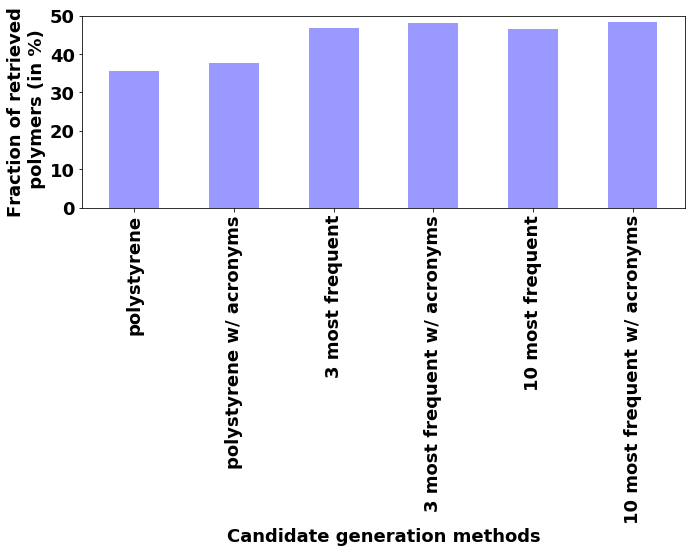
\includegraphics[trim=0in 0.1in 0.1in 0.in,clip,width=1.0\textwidth]{figures/candidate_generation_method1.png}
%\caption{\label{fig:cand_generation1} Fraction of polymer retrieved for various candidate generation methods using most common, three most common and ten most common polymer names as seed entities.
%}
%\end{minipage}\qquad
%\begin{minipage}[b]{.4\textwidth}
%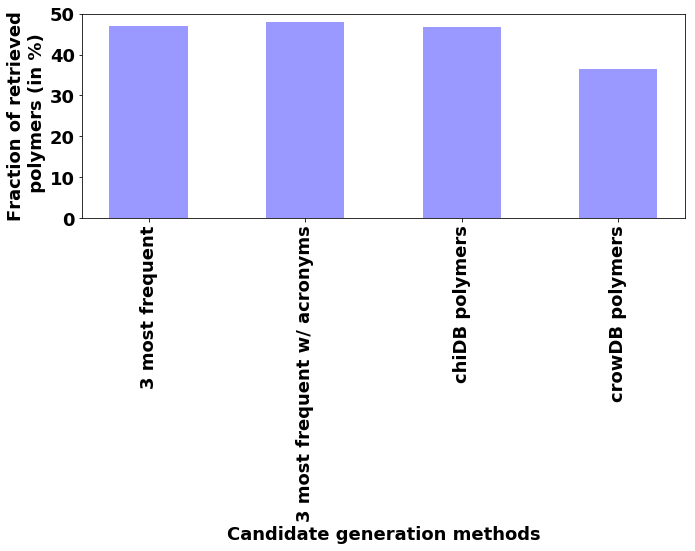
\includegraphics[trim=0in 0.1in 0.1in 0.in,clip,width=1.0\textwidth]{figures/candidate_generation_method2.png}
%\caption{\label{fig:cand_generation2} Fraction of polymer retrieved for various candidate generation methods using three most common (with and without acronymss), $\chi$DB and CrowDB polymer names as seed entities.  
%%\kyle{Not sure this needs to be a separate graph?}
%}
%\end{minipage}
%\end{figure*}
%Together
%[35.55, 37.69, 46.9, 47.97, 46.47, 48.39, 46.68, 36.4]
%[35.55, 37.69, 46.9, 47.97, 46.47, 48.39]
%\begin{figure}[!t]
%\centering
%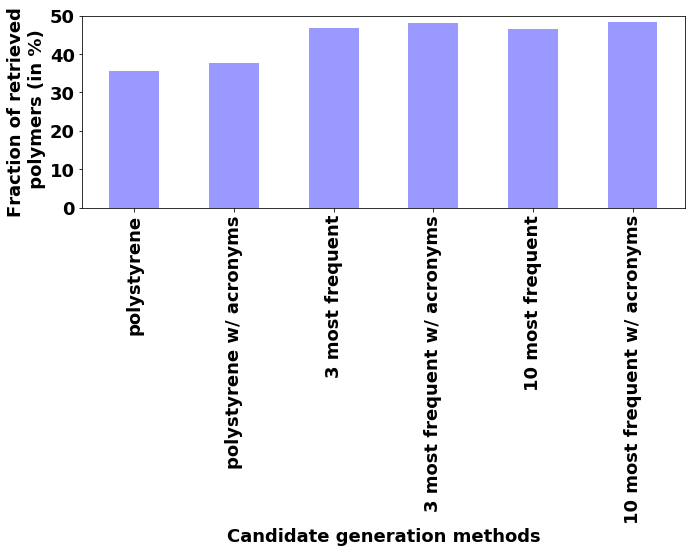
\includegraphics[trim=0in 0.1in 0.1in 0.in,clip,width=3.5in]{figures/candidate_generation_method1.png}
%\caption{\label{fig:cand_generation1} First set of experiments with seed entities showing noticeable improvement from 1 to 3 and less improvement from 3 to 10 seed entities.
%}
%\end{figure}
%[46.9, 47.97, 46.68, 36.4]
%\begin{figure}
%\centering
%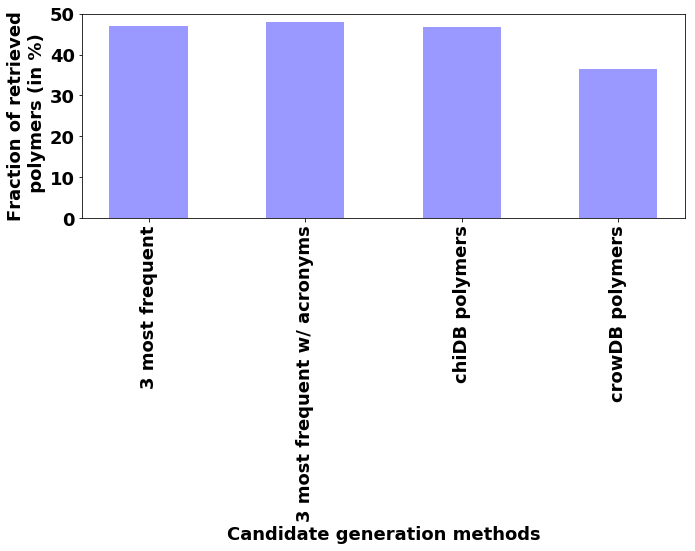
\includegraphics[trim=0in 0.1in 0.1in 0.in,clip,width=3.5in]{figures/candidate_generation_method2.png}
%\caption{\label{fig:cand_generation2} First set of experiments with seed entities showing that using more polymers as seed entities does not necessarily enrich the pool of distance candidates.
%}
%\end{figure}

%\subsubsection{Word Embedding Window and Size Parameters}
%We generate a pool of \num{10000} candidates most similar to the three most frequent polymers and their acronyms from a test corpus of \num{1690}, excluding any token found in our test documents. 
%As previously mentioned, to measure the entity-richness of our dataset, we compute the fraction of polymers retrieved using the distance measure to our representative entities in the  \num{10000} candidates.
%%We measure the impact of the \textit{window} and \textit{size} on the fraction of polymers extracted from the gold standard in the list of \num{10000} candidates most similar to our representative entities. 
%%\logan{Where are the 10k candidates from again? Could we reference this set by its purpose rather than its size?}\roselyne{Done I think.}
%%\logan{Need a reason why this is important? Also, this statement again raises my concern about using "fraction extracted from gold standard" as a metric for quality of the initial training set?}\roselyne{same answer as above, trying to increase balance in dataset.}
%The \textit{window} represents the maximum distance between the current and predicted word within a sentence. In other words, it represents the number of words before and after each word considered by the neural network to generate a vector representation for that word. 
%For each parameter setting, we measure the yield of polymers ten times for each window and vector size setting.
%We observe slightly higher fraction of polymers retrieved for window sizes of 1 and 2. The yield subsequently decreases and more noticeably with window size larger than 5 (see Figure~\ref{fig:window_size}).
%The \textit{size} determines the size of the word vector (features for our classifier).
%We varied this parameter between 100 and 500.
%The average yield of polymer names was measured at 49.3 with a standard deviation of less than 1\% (see Figure~\ref{fig:vector_size}).
%We conclude that the vector size does not impact the fraction of polymers retrieved during the distance candidate generation.
%[49.67880085653105, 49.25053533190578, 49.46466809421842, 49.46466809421842, 48.82226980728051]
%\logan{Need a concluding sentence?}

%\begin{figure}
%\centering
%%\begin{minipage}[b]{.4\textwidth}
%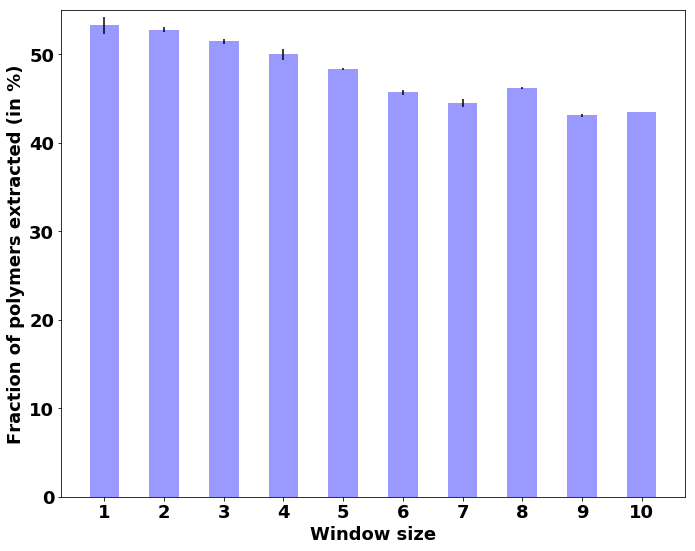
\includegraphics[trim=0in 0.1in 0.1in 0.in,clip,width=3.5in,height=2.5in]{figures/window_size.png}
%\caption{Impact of varying window size on fraction of polymers retrieved.}\label{fig:window_size}
%%\end{minipage}\qquad
%%\begin{minipage}[b]{.4\textwidth}
%%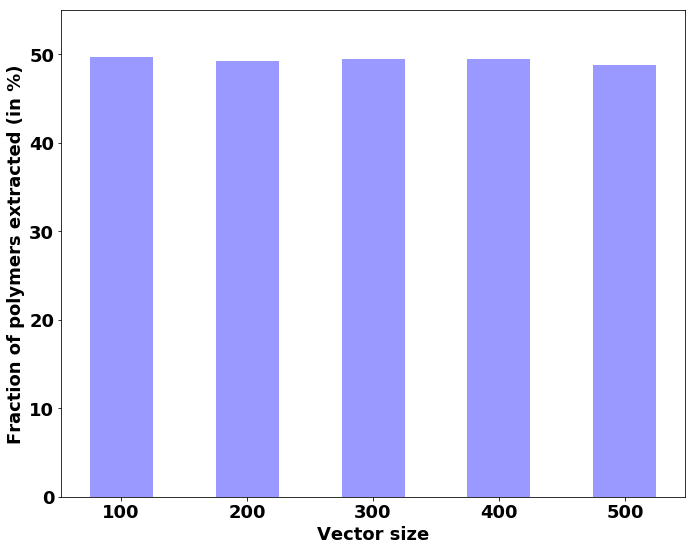
\includegraphics[trim=0in 0.1in 0.1in 0.in,clip,width=1.0\textwidth]{figures/vector_size.png}
%%\caption{Impact of varying vector size on fraction of polymers retrieved. \logan{Can we combine this with F\ref{fig:window_size}? (If we keep it) }}\label{fig:vector_size}
%%\end{minipage}
%\end{figure}
 %\kyle{Not sure this fig is worth including}\roselyne{Agreed that it's not so interesting but i think it goes with the windows one and i will combine the two figures you think should be together.}\roselyne{May remove as paper gets longer}

%\roselyne{We can put labeling here, or maybe before last results, but I think it should be before the discussion and the final main result}
\subsection{Labeling}\label{sec:labeling}
We conduct some experiments to estimate labeling time. 
We ask two polymer scientists to label 200 candidates from a subset of our corpus.
One expert reports 30 minutes, the other 45 minutes. We overestimate the time to label 200 candidates at one hour of expert time.
Based on user feedback, we also improve the labeling Web interface after the above mentioned test rounds to further facilitate and speed up labeling.
For example, we increase the number of example sentences available to provide context, to decrease the number of occurences in which experts have to look up original publications for candidates.
We also increase the size of checkmarks to make it easier to reject erroneous candidates.
%Having performed these initial tests, and considering that expert time is expensive, we allow annotators to save their progress and come back to labeling anytime within a week's time. \roselyne{Is this only going to add confusion?}
In the initial labeling round, 
we perform crosschecking for 10\% of the batch of labels. 
We confirm agreement between labels for all but one of 20: an agreement rate of 95\%.

\subsection{The Initial Classifier}
Recall from Section~\ref{sec:bootstrap} that we use an initial set of 200 NLP-filtered entities that are close
to seed entities to bootstrap our labeling process.
Once those data are labeled by our experts, 
we use 80\% to train a KNN classifier, validating on the remaining 20\%. 
We then test this \textit{initial classifier} against all \num{9656} NLP-filtered candidates in the 100-document test set,
which as noted in Section~\ref{sec:dataset} contain \num{467} polymers.
Results are shown in Figure~\ref{fig:knn_init}.
Its Receiver Operating Characteristic (ROC) curve
shows better-than-random behavior, with an area under curve (AUC) of 0.62. 
 %shows the Receiver Operating Characteristic (ROC) curve for the initial classifier with highest recall when evaluating on the test corpus.
%\logan{I do not like this as a topic sentence because it doesn't offer any indication of what to draw from the figure. I prefer ones that are "We found that X, as shown in Figure Y." Topic sentences with some editorial comments worked in help keep the narrative of the purpose of your study alive.}
%The ROC plot is an evaluation measure that is based on two basic evaluation measures: specificity (true positive rate) and sensitivity (true negative rate).
%Sensitivity is the same as recall. Specificity is a measure of the true negative rate (the proportion of actual negatives that are correctly identified as such).
%A classifier with the random performance level always has the same true positive rate and false negative rate.
%%\logan{Not true. The TPR depends on how many points you sample, and is always equal to the FPR}\roselyne{oh right.}
%A classifier with the perfect performance level shows a combination of two straight lines immediately showing a true positive rate of 1.0 and remaining there as recall increases.
%Classifiers with better-than-random performance levels usually lie in the area between the random ROC curve (baseline) and the perfect ROC curve.
%\logan{Also not quite correct. All classifiers with better-than-random performance lie between random and perfect. Maybe just skip the notion of betweenness and talk about the AUC}\roselyne{this is what I tried to say, you don't like the word meaningful? I meant if it's below it's usually bad.}
%The area under the curve (AUC) measures the area under the ROC.
%Ideally the AUC of a learning algorithm is above 0.5. 
AUC can be misleading for imbalanced datasets, 
as it considers true negatives or correctly predicted non-polymers (inverse ratio).
For example, if a dataset contains 90\% of class A and 10\% of class B, 
a classifier that predicts every sample as belonging to class A has an accuracy of 90\%, 
but is not useful in practice.
%Since AUC takes into account true negatives or correctly predicted non-polymers and our dataset is imbalanced containing more non-polymers than polymers, 
Therefore, we also plot the Precision Recall (PR) curve to show the tradeoff between precision and recall.
While the AUC for the initial classifier is above random performance (0.5) 
its PR curve shows poor precision, regardless of recall.
In previous work~\cite{tchoua2019polyner}, we found that we could 
achieve better performance with more labels (897), suggesting that a KNN classifier begins to learn with more data. 
However, 160 labels (80\% of 200) is not yet enough. % training data to perform well in practice.
%\logan{Better topic sentence. It provides a hit of what to look for. But, you do not follow it up with any details supporting this claim}\roselyne{yes this is where i was doing some explaining for the paragraph, will elabotate}
%\logan{This is a long section for just describing how you made the classifier and that it is pretty bad. Do we need this section?}\roselyne{I will shorten and improve next, the main reason for poor performance is small sample data, because we know this works better with 800 data points, from previous polyNER paper.}

\ian{What do you think about adding the initial classifier lines to Figure~\ref{fig:rocs_prcs_round5}?
It will be more crowded, but the comparison will be clearer.} 

\begin{figure*}
\centering
\begin{minipage}[b]{.4\textwidth}
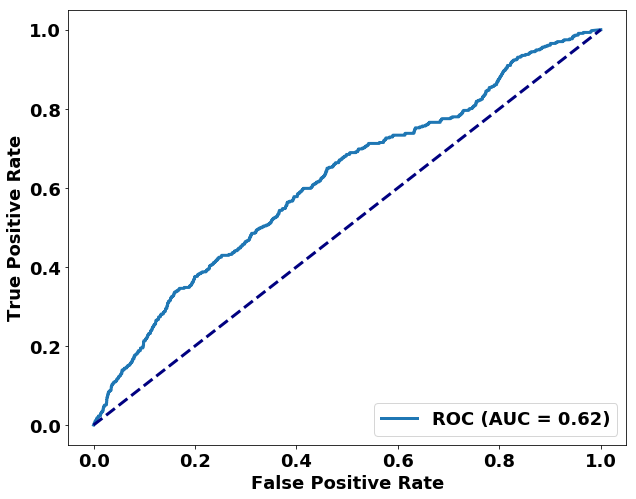
\includegraphics[trim=0in 0.1in 0.1in 0.in,clip,width=1.0\textwidth]{figures/roc_init.png}
\end{minipage}\qquad
\hspace{2ex}
\begin{minipage}[b]{.4\textwidth}
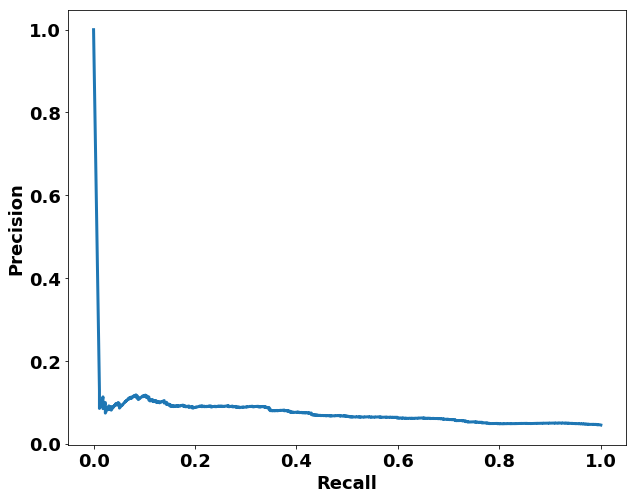
\includegraphics[trim=0in 0.1in 0.1in 0.in,clip,width=1.0\textwidth]{figures/prc_init.png}
\end{minipage}
\caption{ROC (left) and PR (right) curves for KNN model for the initial classifier. 
The PR curve shows that precision is low regardless of recall, 
indicating that we need more data.\label{fig:knn_init}}
\end{figure*}

\begin{figure*}
\centering
\begin{minipage}[b]{.4\textwidth}
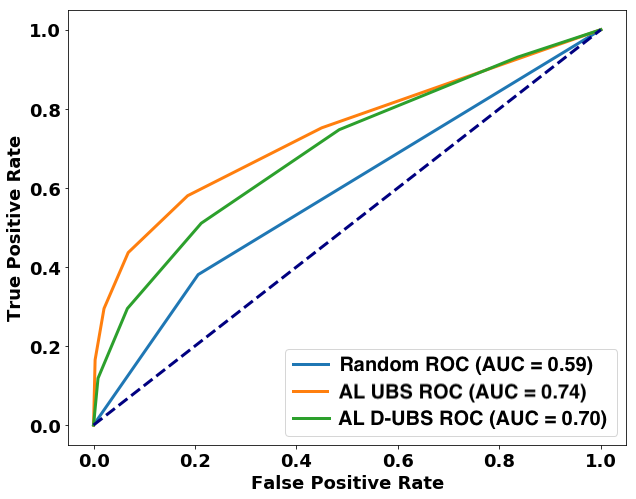
\includegraphics[trim=0in 0.1in 0.1in 0.in,clip,width=1.0\textwidth]{figures/rocs_round5_new.png}
\captionsetup{labelformat=empty}
\label{fig:rocs_round5}
\end{minipage}\qquad
\hspace{2ex}
\begin{minipage}[b]{.4\textwidth}
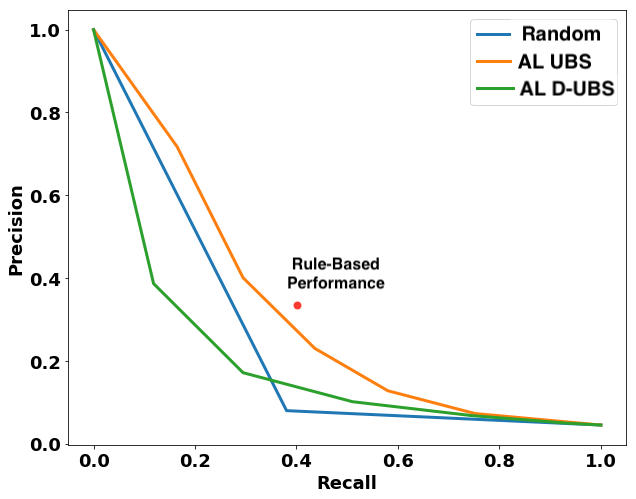
\includegraphics[trim=0in 0.1in 0.1in 0.in,clip,width=1.0\textwidth]{figures/prcs_round5_rule.png}
\captionsetup{labelformat=empty}
\end{minipage}
\caption{ROC (left) and PR (right) curves after four rounds. 
The ROC curves for two active learning strategies, UBS and Distance UBS, show significant improvements,
achieving AUCs of 0.74 and 0.70, respectively: significantly better than the 0.62 achieved by the initial
classifier in Figure~\ref{fig:knn_init}. 
Random, in contrast, performs poorly, with an AUC of just 0.59.
%\ian{I don't understand what you mean here. It is doing better than random. It seems to me that, in general, you are using this graph to make a number of assertions about improvement over initial performance that are not supported by the graph, because you do not show the lines for ``initial performance." All the graph shows is that they all do better than random, with UBS better than Distance UBS, which is in turn better than Random.} 
PR curves also show improvements relative to the initial classifier, with all three strategies
lifting away from the bottom corner, indicating discriminative capacities.
In both types of plots, UBS outperforms Distance UBS. % and approaches rule-based performance.
% AL-1 refers to active learning using NLP-filtered nouns. AL-2 refers to active learning using candidates deemed similar to representative entities.  %\logan{<soapbox>Is it standard practice to use such uninformativ figure captions in CS? I was taught to make the captions almost standalone from the text</soapbox>}
%\ian{I commented out the text that UBS ``approaches rule-based performance'' because the figure does not show that:
%it has no information about rule-based performance.}\roselyne{right! If I add the point, I'll put it back}
}\label{fig:rocs_prcs_round5}\label{fig:prcs_round5}
\end{figure*}

\subsection{Comparing Sampling Strategies}
After the initial round of labeling, we experiment with the three sampling strategies described in Section~\ref{sect:apner_architecture}: Random, UBS, and Distance UBS,
performing four rounds of active learning for each.
Results, in Table~\ref{tab:pr_table}, show
no improvement in the first two rounds for any strategy: % of active learning or the first three rounds of labeling. 
precision remains under 5\% for all.
However, in the third round, we observe increases in precision,
an improvement that  
is sustained in the fourth round for UBS.
Figure~\ref{fig:rocs_prcs_round5} shows ROC and PR curves for the three strategies after four rounds. 
The AUC for UBS is 0.74 and that of Distance UBS is 0.70. 
The PR curves for both are improved (lifting away from the lower left corner of the graph) over the first round, 
with active learning performing better with UBS than with Distance UBS.
%After round 3 and 4, we observe and confirm some, albeit moderate, level context-based predictive ability.
%We also determine that the classifier, which uses UBS is performing better than with the two other strategies.
When tested against our gold standard of 467 one-word polymer names, 
the KNN classifier achieves 18.2\% precision and  45.6\% recall. 

We conclude that while the sampling step
helps insure that the classes are balanced in the initial batch of labels, 
restricting ourselves to just distance candidates, as is done by Distance UBS, does not yield better results than using active learning with all NLP-filtered candidates (UBS).
Intuitively, basic UBS can find \textit{useful} instances (target and non-targets) to be labeled from the entire word embedding space, 
while examples from Distance UBS are clustered around the seed entities that may be collocated in that space.

%\logan{I think the table would be better suited as a plot}\roselyne{I am tempted to remove it, and just indicate that there was not much learning in the first 3 rounds, but Kyle had a comment that people like to see it for themselves and suggested a table. I don't think the plots would look good either has it will bring attention to the problem of using multiple classifiers as previously discussed. I can go back to ommitting this or displaying the last two rounds.}
%\loganfussingaboutrecallandprecision \roselyne{I actually read that this is what people use many times for imbalanced datasets, but I get the point and we have ROCS to got with the last two rounds}

\begin{table}[ht!]
\centering
\caption{Precision and recall relative to the gold standard for
the initial classifier (round 0) and the classifiers trained also with the increased data obtained in each of
four learning rounds, 1--4.\label{tab:pr_table}
}
\vspace{2ex}
%[35.55, 37.69, 46.9, 47.97, 46.47, 48.39, 46.68, 36.4]
\setlength\tabcolsep{6pt}
%\begin{tabular}{*4c}
\begin{tabular}{|c| l | r | r | r |}
\hline
& & \multicolumn{3}{c|}{\textbf{Strategy}} \\
 \textbf{Round} & \textbf{Metric} & \textbf{Random} & \textbf{UBS}  & \textbf{Distance UBS}  \\
%\hline
%Round 0\ \ & \multicolumn{3}{c|}{} \\
\hline
\multirow{2}{*}{0} & Precision &        \multicolumn{3}{c|}{6.53\%} \\
 & Recall\ \ \ \ \ &               \multicolumn{3}{c|}{19.10\%} \\
%\hline
%Round 1\ \  & \multicolumn{3}{c|}{} \\
\hline
\multirow{2}{*}{1}  & Precision     & 3.75\%       &      3.18\%      &  \textbf{5.28\%} \\
 & Recall\ \ \ \ \ & 0.29\%      &   \textbf{93.62\%}     &  56.81\% \\
%\hline
%Round 2\ \  & \multicolumn{3}{c|}{} \\
\hline
\multirow{2}{*}{2} & Precision      & 1.49\%           &      3.79\%      &  \textbf{5.35\%} \\
& Recall\ \ \ \ \ & 1.45\%           &    \textbf{46.38\%}      &  10.14\% \\
%\hline
%Round 3\ \  & \multicolumn{3}{c|}{} \\
\hline
\multirow{2}{*}{3}  & Precision      & 6.02\%              &    \textbf{21.23\%}      &  3.93\% \\
 & Recall\ \ \ \ \ & 44.64\%            &    40.00\%      &  \textbf{84.35\%}  \\
%\hline
%Round 4\ \  & \multicolumn{3}{c|}{} \\
\hline
\multirow{2}{*}{4} & Precision     & 7.06\%          &    \textbf{18.21\%}      &  7.20\% \\
& Recall\ \ \ \ \ & 40.70\%         &     45.64\%     &  \textbf{51.88\%} \\
\hline
\end{tabular}
\end{table}

We selected seed entities based on their frequency in our corpus. %and the yield of target entities during sampling.%\ian{I thought that you said above that you picked the most frequent words?}\roselyne{Yes, but we also experimented with them, top, vs, top3, vs top10, but it is not necessary.}
This observation suggests that we could also study how the choice of seed entities impact of the performance of the classifier during the active learning process. 
We revisit this concept of \textit{diversity} of labels in the Section~\ref{sec:discussion}. 
Note that with limited training data and based solely on context, the classifier retrieves 45.6\% (more than one third) of the gold standard polymers with a precision of 18.2\%, after five hours of expert labeling. 
For comparison, an attempt to extract polymer names using the rule: 
\textit{if the name contains ``poly'' extract it as a polymer}, gets recall of 41\% and precision of 34\% on the same dataset.
We conclude that with our relatively small dataset, we are able to achieve close to rule-based performance, 
using active learning and little labeling.
%\logan{I think we should show this point on the plot for context. Also, state what you conclude from the comparison. Don't leave it up to the reader to state the conclusion.}

%\subsection{Using Active Learning Labels with Character-Level Enhanced Embeddings}
\subsection{Active Learning Labels + Character-Level Embeddings}
\label{sec:results}
After just 1000 labels, the context-based classifier using active learning applied to NLP-filtered candidates achieved performance comparable to rule-based performance, 
but not quite to the polymer-enhanced CDE+.
With the goal of further improving polyNER performance,
we experiment with the use of an alternative word embedding model, FastText, which 
%Next, we train a word embedding model enhanced with sub-word information using polyNER labels. 
%\logan{Why are you doing this? You need some motivation for this section, otherwise it kinds of jumps out of nowhere and begs the question: Why did you not use this through the entire study? Maybe you can say this section is devoted to "further tuning the model now that you have a large-enough pool of data to make selections statistically-reasonable"?}
%We compare the performance to a state-of-the-art chemistry-aware NLP toolkit. 
%and we end with a discussion of the results.
uses word representations enriched with sub-word (character-level) information.
Because FastText considers sub-word information as well as
context, it can consider word morphology differences, such as prefixes
and suffixes. Sub-word information is especially useful for words for which
context information is lacking, as words can still be compared to morphologically similar
existing words. We set the length of the sub-word used for comparison\textemdash
FastText's \texttt{n_gram} parameter\textemdash to five characters, based on our intuition that
many polymers begin with the prefixes ``poly'' or ``poly(.'' 
Therefore, we generate a FastText word embedding model, 
and generate character-enhanced vectors for our UBS-labeled candidates.

%\ian{Next is confusing to me as (it seems to me) you refer to things in roundabout ways:
%e.g., I am not clear what are ``these candidates'' or what it is that is ``identified as best-performing in previous experiments''.}
Next, we train a KNN classifier using vectors for the candidates labeled through active learning from the NLP-filtered candidates (the active learning strategy identified as best-performing in Figure~\ref{fig:prcs_round5}).
%\logan{Confusing. Is UBS not active learning?}\roselyne{it's the sampling method}
We test the classifier against NLP-filtered nouns from our 100-document test set.
KNN classifier performance improves when using these word vectors, 
achieving 29.7\% precision and 81.9\% recall,
%\logan{Why sow both figures if you say PRC is better.}\roselyne{I will end up taking them off, as I'm now at 12 pages}
%In this case, the classifier achieves 29.7\% precision and 81.9\% recall. 
comparable to those achieved by CDE (see Section~\ref{sec:cde}).
% although as CDE aims to extract all
%chemical compounds, not just polymers, it serves only as a demonstration of an
%alternative approach in the absence of a polymer NER system. % (Note that CDE also extracts properties). 
CDE's recall is high
at 74.5\%, but its precision for polymers is, as expected, low at 8.7\%, as it does not incorporate polymer knowledge. 
%\loganfussingaboutrecallandprecision \roselyne{comes with PRC so should be good here}
In Figure~\ref{fig:UBS_prcs_fasttext}, we show the PR curve for the FastText vector classifier
and also results for the polymer-enhanced CDE+
which achieve 42.2\% precision and 68.3\% recall on the same test set.
%\ian{rewording ok here?}\roselyne{yes}
%We show the PR curve for the FastText vector classifier and the CDE+ performance in Figure
%as shown in Figure~\ref{fig:UBS_prcs_fasttext}.\ian{Is this a good place for figure reference?}
We achieve higher recall than CDE and CDE+ using labels from UBS and FastText vectors 
and in-between (higher than CDE and lower than CDE+)
%\ian{I don't know how to interpret this word.}\roselyne{I thought that would be better "than in-between" precision}
precision.%, with only about five hours of expert labeling.

\subsection{Discussion and Future Work}
\label{sec:discussion}
We have previously used seed entities to bootstrap classifiers of context-based word vectors. 
Using an ensemble of classifiers, polyNER allowed users to tradeoff precision and recall.
In this attempt to improve performance, while efficiently using experts' time, we used active learning to obtain more labels. %\roselyne{Repeating again, may need to remove.}
However, we do not observe an increase of precision over the 5\% fraction of polymers until the third round of active learning with NLP-filtered words (800 labels). 
This suggests that our label batch size is lower than the minimum number of labels necessary to start the learning process.
More detailed study of performance vs. label batch size will help pinpoint the appropriate number of labels and level of bootstrapping required for learning.
We can also ask the following questions: Could we achieve CDE performance classifying only context-based (not character enhanced) representation? If so, how many more iterations would it take? If not, how much do we need to increase and improve our current corpus of \num{1690} documents?

PolyNER achieves CDE performance using labels obtained via active learning (UBS sampling strategy) and FastText vectors.
We attribute the increased performance to the character embedding enhancement, which not only recognizes ``poly'' (and yields more names based on this n-gram comparison), 
but also filters out more anomalous candidates (preceding or following polymer names) generated during tokenization and missed by the filtering steps, 
such as ``\textit{$A_mB_n$}'' and ``\textit{Mw/Mn=1.36}.'' 
In other words, the classifiers of character and (context-based) word embedding vectors perform better than classifiers of only context-based word embedding.
Given this result, one may wonder whether the active learning process itself could benefit from using this enhanced vector embedding. 
To determine whether this is the case,
we repeated the active learning experiment using the entire corpus of NLP-filtered candidates and classifying FastText (enhanced) vectors instead of Gensim vectors at each round. 
However, performance was worse than random.
%the classifier's ROC curve did not achieve CDE performance after five rounds and was below random performance.%\logan{Wasn't it also worse than the randomly-selected words?}\roselyne{yes, but doesn't it make you want to see another figure more}






These results suggest that character-level information enhances classifier performance only once a certain threshold of context information has been captured by the embedding.
We explain this observation as follows. 
In FastText, the portion of the word embedding vector generated by using context varies depending on how much context is available in the entire corpus. 
For words deemed to have enough context, vectors do not include any character-level information. 
At the other extreme, for previously unseen words, the embedding is generated based solely on character n-gram information and comparison to other words in the corpus.
During the active learning process, candidates to be labeled by experts are selected by using maximum-entropy-based uncertainty sampling: that is, words for which prediction probability is similar for target and non-target.
Such candidates are more likely to lack context
and thus have vectors that use mostly character-level information.
%When all or most of the word embedding vector 
As a result, the expert is often presented with nearly identical candidates (e.g., PS13k/PMMA12k, PS214k/PMMA12k, PS31.6k/PMMA12k), which hinders the learning process as these candidates are located in close vicinity in terms of the full (character and context) word embedding space.
In other words, in this full space, while their uncertainty measure is comparable, these examples are not \textit{diverse}, where diversity is a measure of the distance of the examples to each other or previously labeled instances~\cite{brinker2003incorporating}.
One solution to explore in future work would be to impose a diversity constraint on the candidates,
for example by using batch active learning~\cite{settles2009active}.
%\logan{There are batch active learning papers, and surely a review. Cite one so that people do not think you're planning to reinvent such methods.}\roselyne{Definitely planned on adding citation but hadn't reread that part, thanks}
%\logan{This seem more like a "Future Work/Can we do even better!?" section than an actual discussion. Should we rename the section accordingly}


%\begin{figure}[H]
\begin{figure}
\centering
%\begin{minipage}[b]{.4\textwidth}
%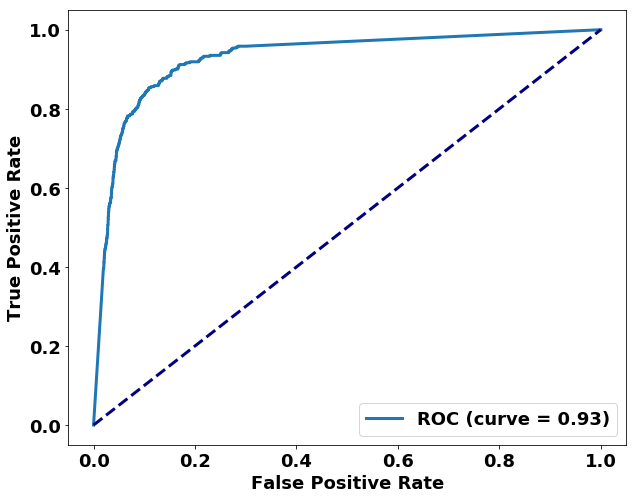
\includegraphics[trim=0in 0.1in 0.1in 0.in,clip,width=3.5in]{figures/fasttext_roc_al_corpus_round5_100}
%\caption{ROC curve for KNN model trained using active learning labels and word representations enriched with character-level information.}\label{fig:UBS_rocs_fasttext}
%\end{minipage}\qquad
%\begin{minipage}[b]{.4\textwidth}
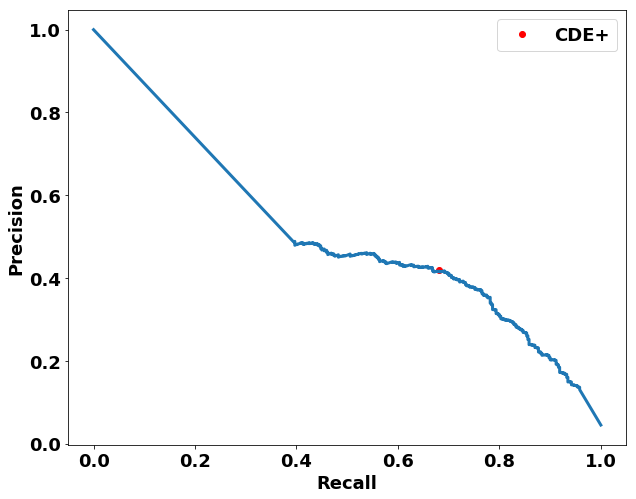
\includegraphics[trim=0in 0.1in 0.1in 0.in,clip,width=3.5in]{figures/fasttext_prc_al_corpus_round5_100}
\caption{PR curve for KNN model trained with active learning labels and word representations enriched with character-level information. Results for CDE+ are also shown.
\ian{I'd be interested in Kyle's views, but I feel that we need some explanation of why the line is straight for recall from 0 to 0.4.}
}
\label{fig:UBS_prcs_fasttext}
%\end{minipage}
\end{figure}

%\subsection{Labeling}\label{sec:labeling}
%We conduct some experiments to estimate labeling time. 
%We ask two polymer scientists to label 200 candidates from a subset of our corpus.
%One expert reports 30 minutes, the other 45 minutes. We overestimate the time to label 200 candidates at one hour of expert time.
%Based on user feedback, we also improve the labeling Web interface after the above-mentioned test rounds to further facilitate and speed up labeling.
%For example, we increase the number of example sentences available to provide context, to decrease the number of occurrences in which experts have to look up original publications for candidates.
%We also increase the size of checkmarks to make it easier to reject erroneous candidates.
%%Having performed these initial tests, and considering that expert time is expensive, we allow annotators to save their progress and come back to labeling anytime within a week's time. \roselyne{Is this only going to add confusion?}
%In the initial labeling round, we
%we perform crosschecking for 10\% of the batch of labels. 
%We confirm agreement between labels for all but one of 20: an agreement rate of 95\%.










%------------------------------------------------------------------------------

%------------------------------------------------------------------------------
\section{Conclusion}
\label{sect:apner_conclusion}
The lack of access to large amount of expert-annotated training data empedes the adoption of recent machine learning techniques in certain scientific applications.
PolyNER is a generalizable system that can efficiently use expert input via approximate candidate generation and active learning for scientific named entity recognition.
We show that using natutal language processing techniques, we can bootstrap a word vector classifier of scientific entities.
PolyNER achieves achieves 31.7\% precision and 82.3\% recall, a performance comparable to well performing
hybrid NER model (CDE+) that combines a dictionary, expert created
rules, and machine learning algorithms and was trained on the CHEMDNER corpus:
a collection of \nistnum{10000} PubMed abstracts that contain a total of 84,355 chemical entity mentions labeled manually by expert chemistry literature curators, following annotation guidelines specifically defined for this task~\cite{krallinger2015chemdner}. 
PolyNER was trained on data annotated using $\sim$ five hours of expert time and minimal untrained crowd input.
While we note that CDE+ is intended to extract polymers and their properties, our work highlights the potential of using minimal amount of data and focused expert input in order to enable machine learning techniques for previously unmined scientific entities. 
We are currently exploring using polyNER-labeled data to annotate text for other NER approaches,
such as bidirectional long short-term memory models.
With a view to exploring generalizability, we are also working to apply polyNER
to quite different problems, such as extracting dataset names from social science
literature. 
%------------------------------------------------------------------------------


% use section* for acknowledgment
\section*{Acknowledgments}
This work was supported in part by NIST contract 60NANB15D077, the Center for Hierarchical Materials Design, and DOE contract DE-AC02-06CH11357, and by computer resources provided by Jetstream~\cite{towns2014xsede,stewart2015jetstream}.
Official contribution of the National Institute of Standards and Technology; 
not subject to copyright in the United States.

\balance
\bibliographystyle{IEEEtran}
\bibliography{references}

% that's all folks
\end{document}
